\begin{frame}{Evolución del recaudo del IVA}
\centering
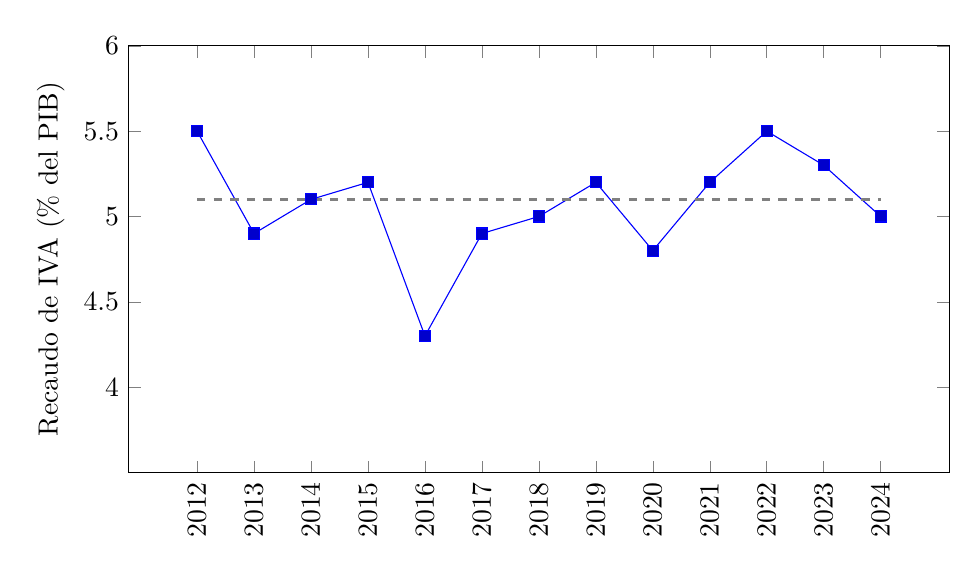
\begin{tikzpicture}
\begin{axis}[
    width=12cm,
    height=7cm,
%    xlabel={Año},
    ylabel={Recaudo de IVA (\% del PIB)},
    ymin=3.5, ymax=6,
    ytick={4,4.5,5,5.5,6},
    xtick={2012,2013,...,2024},
    xticklabel style={rotate=90, anchor=east, /pgf/number format/.cd,1000 sep={}}
]

% Serie de recaudo
\addplot+[mark=square*, solid] coordinates {
(2012,5.5)
(2013,4.9)
(2014,5.1)
(2015,5.2)
(2016,4.3)
(2017,4.9)
(2018,5.0)
(2019,5.2)
(2020,4.8)
(2021,5.2)
(2022,5.5)
(2023,5.3)
(2024,5.0)
};

% Línea punteada del promedio
\addplot[dashed, thick, gray] coordinates {(2012,5.1) (2024,5.1)};

\end{axis}
\end{tikzpicture}
\end{frame}
